% To-Do List %
%   Chapter flow: intros and conclusions

\documentclass[11pt]{report}
\usepackage{StyleSheets/main}
\makeglossaries               % Only makes glossary in main file
\usetikzlibrary{external}     % Allows for cached complitation
\tikzexternalize[prefix=Graphs/tikz/] % Sets cache directory

\begin{document}
\documentclass[11pt]{report}
\usepackage{StyleSheets/main}
\usetikzlibrary{external}     % Allows for cached complitation
\tikzexternalize[prefix=Graphs/tikz/] % Sets cache directory

\begin{document}

\begin{titlepage}

    \tikzset{external/export next=false} % Exclude from externalization
    \begin{tikzpicture}[remember picture, overlay]
        \node[anchor=south east, inner sep=0, opacity=0.05, xshift=100mm, yshift=35mm] at (current page.south east) {
            \includegraphics[width=\paperwidth]{Images/Robot/robot_front_view_greyscale.pdf}  % Adjust only width or height
        };
    \end{tikzpicture}
    
    \centering
    
    \Large{ENGR 2620}
    
    \Large{Integration II}
    
    \Large{Spring 2024}

    \vspace{0.5cm}
    
    \Huge \textsc{\TITLENAME}

    \vfill
    
    \vspace{1cm}
    
    \large{Dr. Jide Williams} \\
    \large{Dr. Irwin Jones}
    
    \vspace{0.8cm}

    \large \textbf{Prepared By:}
    \hspace{1.3cm} \begin{tabular}[t]{@{}l@{}}
        \textbf{Max Westerman}\\
        \textbf{Daniel Carey}\\
        \textbf{Charlie Buttrick}\\
        \textbf{Dylan Wright}\\
    \end{tabular}
    \vspace{10pt}
    
    \vfill
    \hfill \large Report Grade: \underline{\hspace{4cm}}
        
\end{titlepage}

\end{document}


    \begin{tikzpicture}[remember picture, overlay]
        \node[
            anchor=north west,
            fill=gray!20,
            minimum width=\paperwidth,
            minimum height=4cm,
            yshift=-17.35cm,
            xshift = 10.7cm
        ] at (current page.north west) {};
    \end{tikzpicture}

% ---------- %

\microtypesetup{protrusion=false} % Kerning disabled
\singlespacing
\tableofcontents
\listoffigures
\lstlistoflistings
\listoftables
\microtypesetup{protrusion=true} % Kerning Enabled

\newpage
\onehalfspacing

\documentclass[11pt]{report}
\usepackage{StyleSheets/main}
\begin{document}


\chapter{Introduction}\label{ch:introduction}

\hl{Remove personal pronouns such as ``Our''}

This project report goes into depth about a vehicle (also referred to as a system) that has the ability to complete an obstacle course test as well as a pickup and placement test in a multitude of ways. On the obstacle course that is outlined by white lines on the side and green tape on the front and back end, our vehicle will be able to stay within the white lines and detect the walls within the course, maneuver around them, and stop on the green line at the end of the course. For the pickup and placement course, the vehicle will be able to detect an I-Beam, pick up a colored box, and based on its color and size, drop the box off on the other end of the course and return to the starting side of the court. Completing these tests requires communication skills, an array of engineering skills such as computer and electrical skills, writing skills, and decision-making skills. The project intends to strengthen all of the required skills needed to solve a complex problem that meets the demand being asked.

\par The purpose of the report is to detail the process of creating a system that will meet all requirements. The report was also a great way to get the team’s ideas flushed out and catch mistakes within our project that we could then correct. \Cref{ch:project-management-plan} keeps a timeline of the system’s progress by giving weekly updates that include the team member(s) who is responsible for the task and the duration of the task. Another key part of the report is \Cref{ch:system-requirements}. In this part of the report, the system requirements for certain objectives such as the obstacle avoidance and pickup and placement of the vehicle are established. Other major chapters of the report are \cref{ch:conceptual-design,ch:detailed-design}. \Cref{ch:conceptual-design} outlines the conceptual designs that the team came up and \cref{ch:detailed-design} details the design of the system which includes algorithms and other electrical and computer engineering tools that were used in the project. Lastly, \cref{ch:system-test} goes into depth about \gls{TEMPS}. In this chapter, an explanation of how each system requirement is tested is provided.

\end{document}
\documentclass{report}
\usepackage{StyleSheet}
\begin{document}

\chapter{Project Management Plan}\label{ch:project-management-plan}

\end{document}
\documentclass{report}
\usepackage{StyleSheet}
\begin{document}

\chapter{System Requirements}\label{ch:system-requirements}

The overall objective of the system our team has built involves numerous requirements that helped us achieve our objectives. One of the main goals will be for the vehicle to complete the obstacle course in a timely fashion that avoids walls and does not pass specific colored tape. The other main goal will be for the obstacle to pick up a specific colored box, and then follow a particular line of color of the box to a drop-off site, where the vehicle will place the box back down.

\section{Box Pick-up and Placement System}

\subsection{Recognition of the I-Beam}
The vehicle shall find the I-Beam on the course.

\subsection{Orientation of the I-Beam}
The vehicle shall orientate/center itself with the I-Beam

\subsection{Apprehend the Box}
The vehicle shall apprehend the box with the gripper.

\subsection{Identify the Color of the Box}
The vehicle shall identify the color of the box.

\subsection{Identify the Size of the Box}
The vehicle shall identify the size of the box. 

\subsection{Realign with the Line Following Course}
The vehicle shall move itself back onto the line following the course after it has apprehended the box.

\subsection{Follow the Line of the Color of the Box and Return.} 
The vehicle shall follow the colored line of the box’s color it has apprehended.

\subsection{Placement of the Box}
The vehicle shall place the box on the appropriate I-Beam based on the color and size of the box.

\section{Drive Train \& Steering System}

\subsection{Move Forward}
The vehicle shall move forward in a straight line.

\subsection{Move Backward}
The vehicle shall move backward in a straight line.

\subsection{Move Right}
The vehicle shall move right in a straight line.

\subsection{Move Left}
The vehicle shall move left in a straight line.

\subsection{Rotational Movement}
The vehicle shall rotate to the right or left.

\section{Sensor Requirement: IR Sensor Array}

\subsection{Width of the IR Sensors}
The width of the \gls{IR} Array shall be bigger than the width of the tape.

\subsection{The number of sensors is greater than 6}
The amount of sensors on the \gls{IR} Array is greater than 6.

\subsection{It Must Detect and Distinguish the Tape and Tarp}
The \gls{IR} Array must be able to distinguish between the colored tape and the black tarp.

\subsection{It Must be able to Calculate Error}
The \gls{IR} Array must be able to calculate the error to recognize which way the vehicle is deviating.

\subsection{Deviation Adjustment}
The vehicle shall properly correct the vehicle if it deviates from the red, blue, or green line.

\section{Task-2 Completion Times (Obstacle Course)}

\subsection{Detection of Walls }
The vehicle shall detect the walls of the obstacle course via ultrasonic sensors
\subsection{Avoidance of Walls}
The vehicle shall move forward and avoid the walls of the obstacle course by the system not touching any part of the wall. 

\subsection{Detection of Side Boundaries of Obstacle Course via Color Sensors}
The vehicle shall have color sensors that will identify when the system is at the side boundaries of the course. For this specific test, the side boundary is outlined by white tape.

\subsection{Stay within the Obstacle Course Until Course is Complete}
The vehicle’s center of mass shall not deviate outside the side boundary and stay within the obstacle course until completion. 

\subsection{Detection of the Finish Line of Obstacle Course via Color Sensors}
The vehicle shall have color sensors that will identify when the system is at the side boundaries of the course. For this specific test, the side boundary is outlined by white tape.

\subsection{System Stops at the End of the Course}
The vehicle shall detect the green line and fully cross the line, and then stop. 


\end{document}
\documentclass[11pt]{report}
\usepackage{StyleSheets/main}
\begin{document}

\chapter{CONOPs (Concept of Operations)}\label{ch:conops}
The purpose of this section is to provide the user of the robot with a clear and concise description of how this system is operated. The \gls{CONOP}s provides a clear summary of how the vehicle will reach its objective. 
\section{System Summary}
\begin{itemize}
    \item This system is a vehicle with the ability to move right, left, forwards, backwards, and rotate. This vehicle is powered by a battery and controlled using a microcontroller.
    \item The vehicle has a gripper with an arm that allows it to reach for \& pick up objects. 
    \item This vehicle can detect colors, obstacles, and lines.
\end{itemize}
\section{Initialization of the System}
\begin{itemize}
    \item Firstly, the \gls{ABHS} will be placed down on a flat surface, preferably the floor as it takes away the risk of the vehicle falling from a dangerous height.
    \item If the use of the \gls{ABHS} is to fulfill one of its requirements (Obstacle Avoidance, Pickup and Place System with Line Following), then the \gls{ABHS} should be placed in its starting position.
    \item All the connections should be secure and in accordance with the pin map provided with the vehicle.
    \item If a new version of the code is uploaded, verify that the \texttt{while (!Serial)} portion of the \cref{lst:main-h} has been commented out.
    \item Ensure that any external connections the the Teensy 4.1 are terminated to eliminate the possibility of over-powering the Teensy 4.1.
    \item The battery should at this point be connected and switched on, with the green lights appearing when the battery is on. The additional blue \gls{LED} will also light up when the battery is turned on.
\end{itemize}

\section{Standard Operating Modes}
\begin{itemize}
\item This system has 2 normal operating modes:
    \begin{itemize}
        \item This system was designed to perform obstacle avoidance. In the event of a wall being placed in front of the system, the vehicle would find a way around the wall as long as white boundary lines outline the obstacle course.
        \item This system was designed to pick up a box and recognize its color. It will then use this color to transport the box over a line of the same color, and place it in the platform dependant on the size of the box/package. It will then return to its starting position.
\end{itemize}
\end{itemize}
\section {External Environment for use of the System}
\begin{itemize}
    \item This system should typically be used in a room temperature, dry environment. This is due to the open wire nature of the \gls{ABHS}, and its use-case of clean-room operation.
\end{itemize}
\section{Standard Maintenance}
\begin{itemize}
    \item The battery for the \gls{ABHS} should always be charged in order for this system to work.
    \item All wires should be maintained in the correct pin ports. If a wire is in the incorrect port, follow the provided pinout \cref{fig:Pinoutmap}.
    \item The vehicle should be kept in dry, stable conditions, and out of direct sunlight as to avoid potential damage to parts.
\end{itemize}
\section{Failure Modes due to Internal Problems}
\begin{itemize}
    \item In the event of the user at any point seeing or smelling smoke coming from the vehicle, shut the battery off as soon as possible. 
    \item In the case of these events, troubleshoot the system to decipher what the problem point was. Start by seeing if any parts of the system are hot, specifically motors, the Teensy 4.1 microcontroller, and the buck converter. If any signs of overheating occur, immediately disconnect the part for further inspection.
    \item Test the possibly damaged component to see if it functions correctly, if not, replace the damaged component.
\end{itemize}
\section{Reaction to External Failure Modes}
\begin{itemize}
    \item If on the obstacle course the vehicle drives into one of the walls, it should find its own way around it. 
    \item If the vehicle exits the testing course, (ie. over the white line), immediately switch the battery off to avoid the vehicle running too far off course \& potentially crashing, damaging the vehicle.
    \item If during the box pickup test the vehicle drops the box, reset the course and try to run the system again. If this fails again, check to ensure that the gear teeth of the gripper are properly connected.
    \item If the vehicle fails to follow the line and veers off the path, turn off the battery and reset the course. 
\end{itemize}
\section{Shutdown of the System}
\begin{itemize}
    \item Make sure the vehicle has fully run the course of its current objective. Turn the battery off and ensure that the system is fully off. If the vehicle is acting erroneously, it can be manually shut off during it's operation, as it is minimally hazardous to operators.
\end{itemize}


\end{document}
\documentclass{report}
\usepackage{StyleSheet}
\begin{document}

\chapter{Conceptual Design}\label{ch:conceptual-design}

\end{document}
\documentclass[12pt]{report}
\usepackage{StyleSheets/main}
\begin{document}

\chapter{System Risk Management}\label{ch:system-risk-management}

\end{document}

\documentclass{report}
\usepackage{StyleSheet}
\begin{document}

\chapter{Detailed Design}\label{ch:detailed-design}

\end{document}
\documentclass[11pt]{report}
\usepackage{StyleSheets/main}
\begin{document}

\chapter{System Test and Verification}\label{ch:system-test}

{
\footnotesize
\begin{longtable}{|R{2.8cm}|M{2.2cm}|M{2.4cm}|M{2.6cm}|M{0.7cm}|R{3cm}|}
\caption{Verification and Validation Requirements} \label{tab:long_table} \\
\hline \hline
\multirow{2}{3.5cm}{\textbf{Element / Component}} & 
\multirow{2}{*}{\textbf{Requirement}} & 
\multicolumn{3}{c|}{\textbf{Verification \& Validation Methods}} & 
\multirow{2}{3.5cm}{\textbf{Analysis}} \\ \cline{3-5} 
 & 
 & 
\textbf{Inspection} & 
\textbf{Demonstration} & 
\textbf{Test} & 
\\ \hline
\endfirsthead


\multicolumn{6}{c}%
{{\bfseries \tablename\ \thetable{} -- continued from previous page}} \\
\hline
\multirow{2}{3.5cm}{\textbf{Element / Component}} & 
\multirow{2}{*}{\textbf{Requirement}} & 
\multicolumn{3}{c|}{\textbf{Verification \& Validation Methods}} & 
\multirow{2}{3.5cm}{\textbf{Analysis}} \\ \cline{3-5} 
 & 
 & 
\textbf{Inspection} & 
\textbf{Demonstration} & 
\textbf{Test} & 
\\ \hline
\endhead

\hline \multicolumn{6}{|r|}{{Continued on next page}} \\ \hline
\endfoot

\hline \hline
\endlastfoot

% Insert your data here
Box Pickup-and-Placement System & \crefnum{sub:recognition-of-the-i-beam} & \checkmark & & \checkmark & \Cref{tst:location-of-box} -- Location of Box \\
\cline{2-6}
& \crefnum{sub:orientation-of-the-i-beam} & \checkmark & & & \Cref{tst:location-of-box} -- Location of Box \\
\cline{2-6}
& \crefnum{sub:apprehend-the-box} & \checkmark & & \checkmark & \Cref{tst:pickup-of-box} -- Pickup of Box \\
\cline{2-6}
& \crefnum{sub:identify-the-color-of-the-box} & \checkmark & & \checkmark & \Cref{tst:pickup-of-box} -- Pickup of Box \\
\cline{2-6}
& \crefnum{sub:identify-the-size-of-the-box} & \checkmark & & \checkmark & \Cref{tst:pickup-of-box} -- Pickup of Box \\
\cline{2-6}
& \crefnum{sub:realign-with-the-line-following-course} & \checkmark & & \checkmark & \Cref{tst:line-box-following} -- Line Box Following \\
\cline{2-6}
& \crefnum{sub:follow-the-line-of-the-color-of-the-box-and-return} & & & & \Cref{tst:line-box-following} -- Line Box Following \\
\cline{2-6}
& \crefnum{sub:placement-of-the-box} & \checkmark & & \checkmark & \Cref{tst:line-box-following} -- Line Box Following \\
\hline
\multirow{-3}{*}{Drive Train} & \crefnum{sub:move-forward} & \checkmark & & \checkmark & \Cref{tst:basic-directional-movement} -- Basic Directional Movement \\
\cline{2-6}
& \crefnum{sub:move-backward} & \checkmark & & \checkmark & \Cref{tst:basic-directional-movement} -- Basic Directional Movement \\
\cline{2-6}
& \crefnum{sub:move-right} & \checkmark & & \checkmark & \Cref{tst:basic-directional-movement} -- Basic Directional Movement \\
\cline{2-6}
& \crefnum{sub:move-left} & \checkmark & & \checkmark & \Cref{tst:basic-directional-movement} -- Basic Directional Movement \\
\cline{2-6}
\multirow{-2}{*}{Drive Train cont.} & \crefnum{sub:rotational-movement} & \checkmark & & \checkmark & \Cref{tst:rotational-movement} -- Rotational Movement \\
\hline
\multirow{-2}{*}{IR Sensor} & \crefnum{sub:width-of-the-ir-sensors} & \checkmark & & & \Cref{tst:ir-array-observation} -- \gls{IR} Array Observation \\
\cline{2-6}
& \crefnum{sub:the-number-of-sensors-is-greater-than-6} & \checkmark & & & \Cref{tst:ir-array-observation} -- \gls{IR} Array Observation \\
\cline{2-6}
& \crefnum{sub:it-must-detect-and-distinguish-the-tape-and-tarp} & \checkmark & & \checkmark & \Cref{tst:ir-array-detection} -- \gls{IR} Array Detection \\
\cline{2-6}
& \crefnum{sub:it-must-be-able-to-calculate-error} & \checkmark & & \checkmark & \Cref{tst:ir-array-detection} -- \gls{IR} Array Detection \\
\cline{2-6}
& \crefnum{sub:deviation-adjustment} & \checkmark & & \checkmark & \Cref{tst:ir-array-movement} -- \gls{IR} Array Movement \\
\hline
\multirow{-3}{*}{Obstacle Avoidance} & \crefnum{sub:detection-of-walls} & \checkmark & & \checkmark & \Cref{tst:avoidance-of-boundaries-of-walls} -- Avoidance of Boundaries of Walls \\
\cline{2-6}
& \crefnum{sub:avoidance-of-walls} & \checkmark & & \checkmark & \Cref{tst:avoidance-of-boundaries-of-walls} -- Avoidance of Boundaries of Walls \\
\cline{2-6}
& \crefnum{sub:detection-of-side-boundaries-of-obstacle-course-via-color-sensors} & \checkmark & & \checkmark & \Cref{tst:color-sensing-for-side-boundaries} -- Color Sensing For Side Boundaries \\
\cline{2-6}
 & \crefnum{sub:stay-within-the-obstacle-course-until-course-is-complete} & \checkmark & & \checkmark & \Cref{tst:color-sensing-for-side-boundaries} -- Color Sensing For Side Boundaries \\
\cline{2-6}
 & \crefnum{sub:detection-of-the-finish-line-of-obstacle-course-via-color-sensors} & \checkmark & & \checkmark & \Cref{tst:color-sensing-for-end-boundaries} -- Color Sensing For End Boundary \\
\cline{2-6}
 & \crefnum{sub:system-stops-at-the-end-of-the-course} & \checkmark & & \checkmark & \Cref{tst:color-sensing-for-end-boundaries} -- Color Sensing For End Boundary \\
\end{longtable}
\scriptsize
}

\test{Location of Box}\label{tst:location-of-box}
\Cref{sub:recognition-of-the-i-beam,sub:orientation-of-the-i-beam} of the project were put in place to make the vehicle identify where the location of the I-beam is and to align the center of the system with the I-beam so the vehicle shall successfully pick up and place the box. These requirements were verified via inspection by watching the vehicle perform and by testing. The test was a type 2 test. The expected result of this test is that the vehicle shall move forward until the I-beam is detected and the vehicle will center itself in the middle of the I-beam. The vehicle was placed on a black tarp, the front end facing the I-beam. The I-beam is 20 inches in front of the vehicle, slightly off to the vehicle’s left. The USB connected the battery to the Teensy 4.1 board. The \texttt{PickupPlace} code in Arduino was then verified and uploaded. The battery is then turned on and the test begins. 

It was observed that the vehicle deviated off center and once the system detected the I-beam, the vehicle was to the right of the I-beam. The vehicle then moved forward, but it was not centered with the I-beam. The left motor speed was then adjusted slightly and an \gls{IR} sensor array was added to the bottom of the front part of the vehicle. The test was ran again 3 more times and it was observed that the centering of vehicle improved dramatically. However the system’s ability to detect the I-beam was still not meeting standards. It was then decided that using the left and right ultrasonic sensors was not bringing the accuracy and precision that was needed. A middle ultrasonic is then added in front of the front omni-wheel. The test is then ran again and it was observed that rhe vehicle then moved forward and was able to stay on a straight line and once the middle front sensor reached its trigger point it would start. After making these adjustments, the test and \cref{sub:recognition-of-the-i-beam,sub:orientation-of-the-i-beam} were then deemed successful.

\test{Pickup of Box}\label{tst:pickup-of-box}
\Cref{sub:apprehend-the-box} of the project state that the vehicle shall apprehend the box with the gripper. \Cref{sub:identify-the-color-of-the-box,sub:identify-the-size-of-the-box} identifying the color and size of the box also were able to be included in this test. These requirements were verified via inspection by watching the vehicle perform and by testing. The test was a type 2 test. The expected result of this test is that once the vehicle has arrived to the platform, centered itself with the platform, and lowered the gripper arm, the gripper shall apprehend the box and the examiner will be able to tell via the serial monitor the color of the box and the size of the box. Another aspect of this test was making sure the pushbuttons would click when it makes contact with the box. The 2 pushbutton are attached to the inside of the gripper finger clicked. The purpose of the pushbutton were to make sure the gripper finger stopped closing once it had apprehended the box and not squeeze the box. The gripper arm would then rise and the test would be deemed complete.  The blue and red boxes are then held between the fingers of the gripper where a color sensor is placed, and the color sensor is calibrated for the test. The vehicle was placed on a black tarp that has a green line. The vehicle is placed on top of a green line parallel to the I-beam, the front end of the vehicle faced the I-beam. A red box is placed on top of the I-beam. The I-beam is 20 inches in front of the vehicle, slightly off to the vehicle’s left. The USB connected the battery to the Teensy 4.1 board. The \texttt{PickupPlace} code in Arduino was then verified and uploaded. The battery is then turned on and the test begins. 

It is observed that the system moves forward and is centered itself with the I-beam. The gripper arm then lowers, however it does not lower enough that the gripper fingers are in between the box, the gripper fingers then close and the arm raises. The first adjustment that is made is the gripper arm angle. This is a line of code that determine how low or high the gripper arm will go. The gripper arm angle is adjusted and then test is ran again. It is then observed that system moves forward and is centred itself with the I-beam. The gripper arm then lowers the proper amount and the box is between the gripper fingers. The gripper finger closes and picks up the box successfully. It was also observed that the pushbutton did click. Another observation is made via observing the serial monitor on Arduino is that the color sensors and timing algorithm are working properly thus the correct color of the box can be detected and the time it takes the gripper to close can be record. The test is then ran 2 more times to check for consistency and it is observed that both times the pushbutton did not click. An adjustment is then made to the gripper finger which is removing the front pushbutton. The test is then ran 2 more times and 
\cref{sub:apprehend-the-box,sub:identify-the-size-of-the-box,sub:identify-the-color-of-the-box} are all met as well as the consistency of the pushbutton.

\test{Line Box Following}\label{tst:line-box-following}
\Cref{sub:realign-with-the-line-following-course} of the project states that the vehicle shall realign itself with the line following course. This must be done after apprehending the box and identifying the size and color of the box, thus for this test, it is assumed that \cref{sub:recognition-of-the-i-beam,sub:orientation-of-the-i-beam,sub:apprehend-the-box,sub:identify-the-size-of-the-box,sub:identify-the-color-of-the-box} are deemed complete. This test shall also check \cref{sub:follow-the-line-of-the-color-of-the-box-and-return,sub:placement-of-the-box}. These requirements were verified via inspection by watching the vehicle perform the line box following testing. The test was a type 2 test. The expected result of this test is once the vehicle has arrived to the platform, centered itself with the platform, lowered the gripper arm, apprehended the box, and determined the color and size of the box, the system will move backward until it has sensed a green line. It will then center itself over the green line, rotate the front of the vehicle to the side of the line that correlates to the box color, which will be blue or red for this project, and follow the green line to start of the red or blue line. It will then rotate onto the blue or red line and follow it to the other end of the course where it will be place it on a specific I-beam based on the size of the box. The vehicle was placed on a black tarp that has a green line. The vehicle is placed on top of a green line parallel to the I-beam, the front end of the vehicle faced the I-beam. A ‘big’ red box is placed on top of the I-beam. The USB connected the battery to the Teensy 4.1 board. The \texttt{PickupPlace} code in Arduino was then verified and uploaded. The battery is then turned on and the test begins. 

It was observed that the vehicle did arrived to the platform, centered itself with the platform, lowered the gripper arm, apprehended the box, and determined the color and size of the box, the system then moved backward until it has sensed a green line. It then centered itself over the green line, rotated the front of the vehicle to the side of the red line and moved forward on the green line to the beginning of the red line. The rotation onto the red line and its ability to stay straight on the red line was lacking. The system would make it all the way to the fork of the red tape where the red line split into two lines and the vehicle was to follow one of them depending on the size of the box. Once it reached that point it was not able to stop and move horizontally in the proper manner which is key for \cref{sub:placement-of-the-box}. The vehicle was also have issues centering itself over the red line and it was determined as well that the systems ability to consistently put itself over the green line to the standard we expected was not being met. It was then decided that a color sensor needed to be added to the front of the vehicle on the bottom side. This was put in to help center the vehicle on the green, red, and blue lines of tape and identify the fork of the red or blue tape. Another adjustment that was added was to vehicle was vehicle was an \gls{IR} Array. After the color sensor was calibrated and the \gls{IR} array was tested, the line box following test was ran again. It was observed that the vehicle did arrived to the platform, centered itself with the platform, lowered the gripper arm, apprehended the box, and determined the color and size of the box, the system then moved backward until it has sensed a green line. It then centered itself over the green line, rotated the front of the vehicle to the side of the red line and moved forward on the green line to the beginning of the red line. The vehicle then geometrically centered over the red line, rotated onto the red line and did not get off track. It then followed the red line all the way to fork of red tape, stopped when it was supposed to, moved to the right, followed the red tape forward, sensed the I-beam, placed the box back on the I-beam. It then raised the gripper arm slightly, rotated 180 degrees and followed the red line back to the start of the red line. 

\test{Basic Directional Movement}\label{tst:basic-directional-movement}
This test is set up to complete \cref{sub:move-forward,sub:move-backward,sub:move-right,sub:move-left} which are the foundation of the project by being able to move in all directions. These requirements were verified via inspection by watching the vehicle perform and by testing. The test was a type 1 test. The expected result is that the vehicle’s left, right, front, and rear wheel shall rotate forward and backwards half a second each and then after all 4 wheels rotate the vehicle shall move forward for 3 seconds, and stop. Then move backwards for 3 seconds, and stop. It would next move right for 3 seconds, and stop. Then move left for 3 seconds, and stop. The vehicle was placed on the floor. The USB connected the battery to the Teensy 4.1 board. A method in the code, \texttt{motorTest()}, under the class \texttt{Motor}, was then verified and uploaded. The battery is then turned on and the test begins. The code is found in \cref{lst:motor-h}.

It was observed that the vehicle’s left, right, front, and rear wheel rotated forward and backwards half a second each move forward for 3 seconds, and stop. Then the vehicle moved forward for 3 seconds and stopped. It then moved backwards for 3 seconds, and stop. It next moved right for 3 seconds, and stop. Then moved left for 3 seconds, and stop. The test and requirements \cref{sub:move-forward,sub:move-backward,sub:move-right,sub:move-left} were then deemed successful.

\test{Rotational Movement}\label{tst:rotational-movement}
This test is set up to complete \cref{sub:rotational-movement}. This requirements was verified via inspection by watching the vehicle perform and by testing. The test was a type 1 test. The expected result is that the vehicle shall follow a piece of red tape that is straight for the first 2 and a half feet and then veers 45 degrees to the right. The vehicle was placed on a black tarp at the beginning of the red tape, with the front of the vehicle facing the red tape. The USB connected the battery to the Teensy 4.1 board. The code within \gls{IR} class Arduino was then verified and uploaded, seen in \cref{lst:irsensorarray-h}. The battery is then turned on and the test begins. 

It was then observed that the vehicle would move straight forward on the red tape but when it encountered the red tape at the 45 degree angle, the vehicle was over rotating and unable to rotate onto the centerline. One adjustment that was made was to change the speed of the front and back motors. Another change that was made was to the \gls{IR} array sensor and how the vehicle used the error data the array produced. After the test was run 3 more times and the motor speeds were changed, it was observed that the vehicle would move straight forward on the red tape and  then encountered the red tape, it would properly rotate to the center of the red tape at a 45 degree line. Test and \cref{sub:rotational-movement} were deemed complete. 

\test{IR Array Observation}\label{tst:ir-array-observation}
\Cref{sub:width-of-the-ir-sensors,sub:the-number-of-sensors-is-greater-than-6} were completed via inspection. The \gls{IR} Array was scaled against the tape that is used for the courses. It was deemed it was the bigger than the size of the tape in terms of width. The number of sensors was also deemed to be greater than 6. \Cref{sub:width-of-the-ir-sensors,sub:the-number-of-sensors-is-greater-than-6} were completed. 

\test{IR Array Detection}\label{tst:ir-array-detection}
\Cref{sub:it-must-detect-and-distinguish-the-tape-and-tarp} is completed via inspection and testing. The \gls{IR} Array is attached to the button of the vehicle and connected to the Teensy 4.1 board via wires. The expected result of this test is that the vehicle will move as straight as possible on a red line of tape. The serial monitor will be observed at the same time of the vehicle’s movement. It is expected that once the vehicle begins to deviate right or left the values the serial monitor will change from what they were when the vehicle was moving straight. The vehicle is placed at the beginning of a straight piece of red tape, 30 inches long. The USB connected the battery to the Teensy 4.1 board. The \gls{IR} Array Test code is uploaded and verified. The battery is then turned on and the test begins. 

It is observed that the values of the serial monitor are changing when a sensor is over the tape compared to the black tarp. When the left arrays deviate to the left off the red tape their values become less than zero and when the right sensors deviate to the right off the tape, their values are greatest than zero. It is deemed \cref{sub:it-must-detect-and-distinguish-the-tape-and-tarp} is complete. 

\hl{THERE IS NO SUB REQUIREMENT 2.16.1?}

\hl{Sub-requirement 2.16.1} is also completed in this this test by adding code that sums of the average values of the right sensors and add that value to the sum of the left array values. We are able to tell with that value if the vehicle is deviating left of right. If the value is negative it’s beginning to yaw to the left and if the value is positive we know it is beginning to yaw to the right. 

The updated code is verified and uploaded, the test is ran again. The vehicle moved forward on the red line and began to deviate to the left and a negative error was observed on the serial monitor. It was deemed \hl{requirement 2.16.1} is complete. 

\test{IR Array Movement}\label{tst:ir-array-movement}
The \gls{IR} array movement test is set to complete \cref{sub:it-must-be-able-to-calculate-error}. The expected result of this test is that the vehicle shall correct its deviation by turning back onto the line. The test will be on a green, blue, and red line. The rate of how much the vehicle turns is based on the absolute value of the error. The further away the error is from zero the more it will turn. The vehicle is placed at the beginning of a straight piece of red tape, 30 inches long. The USB connected the battery to the Teensy 4.1 board. The \gls{IR} Array deviation Test code is uploaded and verified. The battery is then turned on and the test begins. 

It is observed that the vehicle moved forward and deviated to the right and gave an error value of 0.4 when it began to drift to the right. It was then observed however that the amount the system corrected itself to the left was not enough thus it did not put itself back on the red tape. It was then decided that the proportional gain needed to be adjusted by increasing the value. The code was then updated and the test was then ran again. This test run the system drifted to the left and the error value as it first began to deviate from the line was -0.2, it then corrected it path by the correct amount of rotation. This was then tested on a green and blue line as well and no issues were found. \Cref{sub:it-must-be-able-to-calculate-error} was deemed complete


\test{Avoidance of Boundaries of Walls}\label{tst:avoidance-of-boundaries-of-walls}
\Cref{sub:detection-of-walls,sub:avoidance-of-walls} of the project were put in place to make the vehicle avoid all walls within the obstacle course. These requirements were verified via inspection by watching the vehicle perform and by testing. The test was a type 2 test. The expected result of this test is that the vehicle will move forward until a wall is detected at a trigger distance, then move left until the right sensor senses a gap. It will then move forward until a wall is detected at trigger distance and then move left again. It is also expected that the vehicle stays in a straight line when moving horizontally. The test would then be deemed complete. The vehicle was placed on a black tarp, the front end facing the obstacle course. Two walls were placed on the obstacle course, one on the left side and one on the right side, about 30 inches apart vertically.  The USB connected the battery to the Teensy 4.1 board. The obstacle code in Arduino was then verified and uploaded. The battery is then turned on and the test begins. 

It was observed that the vehicle would move forward property, move left properly, stay in a straight line when moving horizontally, and not hit the wall or obstacle when moving forward, however when a gap was sensed it would wait too long to move forward. This was then fixed by reducing the motor speed and decreasing the delay. After making these adjustments, the test and \cref{sub:detection-of-walls,sub:avoidance-of-walls} were then deemed successful.

\test{Color Sensing For Side Boundaries}\label{tst:color-sensing-for-side-boundaries}
\Cref{sub:detection-of-side-boundaries-of-obstacle-course-via-color-sensors} was tested in the color sensing test for the side boundaries. This requirement was verified via inspection by watching the vehicle perform and by testing. The test was a type 2 test. The expected result of this test is that it would move forward from the starting position, detect a wall, and then move left until it detected a white line and move in the opposite direction which would satisfy \cref{sub:stay-within-the-obstacle-course-until-course-is-complete}. The vehicle was placed on a black tarp, the front end facing the obstacle course. Two walls are placed side by side about 20 inches from the starting position. The USB connected the battery to the Teensy 4.1 board. This test assumes \hl{test 4.1} and \cref{sub:detection-of-walls,sub:avoidance-of-walls} are completed. The obstacle test code which includes the color sensing code and obstacle avoidance code in Arduino was then verified and uploaded. The battery is then turned on and the test begins.

It was then observed that the vehicle moved forward, detected a wall, and moved left until a white line was detected, however, the vehicle then oscillated over the white line and did not have the ability to move back to the right. It was then discovered that the color sensors did not clear the data from the previous loop of code and since this code was using average color values the sensor had seen, it was then realized the data needed to be cleared so it wouldn’t affect the next task. This adjustment was made to the code. The test was then run again in the same form. It was then observed that the vehicle moved forward, detected a wall, and moved left until a white line was detected then moved back to the right side of the obstacle course, detected a white line, and moved back to the left. After making these adjustments, the test and \cref{sub:detection-of-side-boundaries-of-obstacle-course-via-color-sensors} were then deemed successful.

\test{Color Sensing for End Boundaries}\label{tst:color-sensing-for-end-boundaries}
\Cref{sub:detection-of-the-finish-line-of-obstacle-course-via-color-sensors,sub:system-stops-at-the-end-of-the-course} was tested in the color sensing test for the end boundary. This requirement was verified via inspection by watching the vehicle perform and by testing. The test was a type 2 test. The expected result of this test is that it would move forward from the starting position, detect a green line, and then fully cross the green line where it would come to a complete stop which would satisfy \cref{sub:system-stops-at-the-end-of-the-course}. The vehicle was placed on a black tarp, about 15 inches from the end of green tape/end of the course. The USB connected the battery to the Teensy 4.1 board. The obstacle test code which includes the color sensing code in Arduino was then verified and uploaded. The battery is then turned on and the test begins.

It was then observed that the vehicle moved forward, and detected a green line, however, the vehicle then only moved about halfway across it. \hl{A delay function and a variable named VerticleBoxLength were added to the code to make the vehicle fully cross the line in a more accurate manner.} The test was then run again and the vehicle detected a green line and fully crossed the line and then came to a complete stop. \Cref{sub:system-stops-at-the-end-of-the-course,sub:detection-of-the-finish-line-of-obstacle-course-via-color-sensors} were fulfilled, thus a successful test. 

\end{document}
\documentclass[12pt]{report}
\usepackage{StyleSheets/main}
\begin{document}

\chapter{System Analysis \& System Performance Metrics}\label{ch:system-analysis}

\end{document}
\documentclass{report}
\usepackage{StyleSheet}
\begin{document}

\chapter{Summary}\label{ch:summary}

\end{document}

\singlespacing
\microtypesetup{protrusion=false} % Kerning disabled
\printglossary[type=\acronymtype]
\microtypesetup{protrusion=true}  % Kerning Enabled

\appendix

\section*{Documentation Statement}
\begin{description}
    \item[Speed Motor \#1:] To make the robot faster, the gearboxes of dead speed motors were swapped out with our slower, torque motors. The team utilized \emph{Savannah Prouty's} dead speed motor.
    \item[Speed Motor \#2:] As above, the team utilized \emph{Duncan Wood's} dead speed motor for it's gearbox.
    \item[\gls{PID} Guidance:] Although it did not make it into the final robot, \emph{Carter Sorenson} introduced the group to the possibility of using \gls{PID} control for the robot.
    \item[Motor Mounts:] The team did not check our box correctly, resulting in missing motor mounts. \emph{Savannah Prouty} provided the team with her extra motor mounts.
\end{description}

\documentclass[12pt]{report}
\usepackage{StyleSheets/main}
\begin{document}

\chapter{Calibration Data}\label{ch:calibration-data}

\section{Color Sensor Calibration Points}
\label{sc:color-sensor-points}
\documentclass{article}
\usepackage{GraphDefinitions}

\begin{document}

\foreach \sensor in {middleColor, rightColor, leftColor, gripperColor} {
    \ifthenelse{\equal{\sensor}{middleColor}}{ % Middle color shadow opacity
        \def\opacity{0.010}
    }{
        \def\opacity{0.055} % Non middle color shadow opacity
    }
    \def\ballsize{3pt} % Change the size of the balls
                
    \begin{figure}[H]
        \centering
        \begin{tikzpicture}
            \begin{axis}[
                xlabel={Red Frequency},
                ylabel={Green Frequency},
                zlabel={Blue Frequency},
                xlabel style={sloped like x axis}, % Make x label follow the x axis
                ylabel style={sloped like y axis}, % Make y label follow the y axis
                zlabel style={sloped}, % Make z label follow the z axis or make it vertical
                legend pos=north west,
                grid=both,
                grid style={line width=.1pt, draw=gray!10},
                major grid style={line width=.2pt,draw=gray!50},
                minor tick num=5,
                width=0.8\textwidth,
                height=0.65\textwidth,
                view={45}{45}, % Adjust the view angle for better visualization
            ]
            \IfFileExists{code/output_data/color_sensor_calibration/\sensor.csv}{
                % Determine opacity based on sensor

                \addplot3[
                    only marks,
                    scatter,
                    scatter/classes={
                        RED={mark=ball,ball color= red, draw opacity=0, mark size = \ballsize},
                        BLUE={mark=ball,ball color= blue, draw opacity=0, mark size = \ballsize},
                        GREEN={mark=ball,ball color= green, draw opacity=0, mark size = \ballsize},
                        WHITE={mark=ball,ball color= white, draw opacity=0, mark size = \ballsize},
                        BLACK={mark=ball,ball color= black, draw opacity=0, mark size = \ballsize},
                        YELLOW={mark=ball,ball color= yellow, draw opacity=0, mark size = \ballsize}
                    },
                    scatter src=explicit symbolic,
                ] table[
                    x=Red_Freq,
                    y=Green_Freq,
                    z=Blue_Freq,
                    meta = Color,
                    col sep=comma,
                ] {code/output_data/color_sensor_calibration/\sensor.csv};

                % Wall histogram on the left
                \addplot3[
                    only marks,
                    scatter,
                    scatter/classes={
                        RED={mark=*,fill=red, fill opacity=\opacity, draw opacity=0},
                        BLUE={mark=*,fill=blue, fill opacity=\opacity, draw opacity=0},
                        GREEN={mark=*,fill=green, fill opacity=\opacity, draw opacity=0},
                        WHITE={mark=*,fill=gray, fill opacity=\opacity, draw opacity=0},
                        BLACK={mark=*,fill=black, fill opacity=\opacity, draw opacity=0},
                        YELLOW={mark=*,fill=yellow, fill opacity=\opacity, draw opacity=0}
                    },
                    scatter src=explicit symbolic,
                ] table[
                    x expr = 0,  % This sets the x-coordinate to 0
                    y = Green_Freq,  % This sets the y-coordinate to 0
                    z= Blue_Freq,
                    meta = Color,
                    col sep=comma,
                ] {code/output_data/color_sensor_calibration/\sensor.csv};

                % Wall histogram on the right
                \addplot3[
                    only marks,
                    scatter,
                    scatter/classes={
                        RED={mark=*,fill=red, fill opacity=\opacity, draw opacity=0},
                        BLUE={mark=*,fill=blue, fill opacity=\opacity, draw opacity=0},
                        GREEN={mark=*,fill=green, fill opacity=\opacity, draw opacity=0},
                        WHITE={mark=*,fill=gray, fill opacity=\opacity, draw opacity=0},
                        BLACK={mark=*,fill=black, fill opacity=\opacity, draw opacity=0},
                        YELLOW={mark=*,fill=yellow, fill opacity=\opacity, draw opacity=0}
                    },
                    scatter src=explicit symbolic,
                ] table[
                    x = Red_Freq,  % This sets the x-coordinate to 0
                    y expr = 750,  % This sets the y-coordinate to the back wall
                    z= Blue_Freq,
                    meta = Color,
                    col sep=comma,
                ] {code/output_data/color_sensor_calibration/\sensor.csv};

                % Floor histogram
                \addplot3[
                    only marks,
                    scatter,
                    scatter/classes={
                        RED={mark=*,fill=red, fill opacity=\opacity, draw opacity=0},
                        BLUE={mark=*,fill=blue, fill opacity=\opacity, draw opacity=0},
                        GREEN={mark=*,fill=green, fill opacity=\opacity, draw opacity=0},
                        WHITE={mark=*,fill=gray, fill opacity=\opacity, draw opacity=0},
                        BLACK={mark=*,fill=black, fill opacity=\opacity, draw opacity=0},
                        YELLOW={mark=*,fill=yellow, fill opacity=\opacity, draw opacity=0}
                    },
                    scatter src=explicit symbolic,
                ] table[
                    x = Red_Freq,
                    y = Green_Freq,
                    z expr = 0,
                    meta = Color,
                    col sep=comma,
                ] {code/output_data/color_sensor_calibration/\sensor.csv};

                
            }{}
            \end{axis}
        \end{tikzpicture}
        \caption{\sensor \ Sensor Calibration Data in Euclidean Space.}
        \label{fig:\sensor_calibration_data}
    \end{figure}
}

\end{document}

\section{IR Array Calibration Points}
\label{sc:ir-array-points}
\documentclass{article}
\usepackage{GraphDefinitions}

\begin{document}

\begin{figure}[H]
\centering
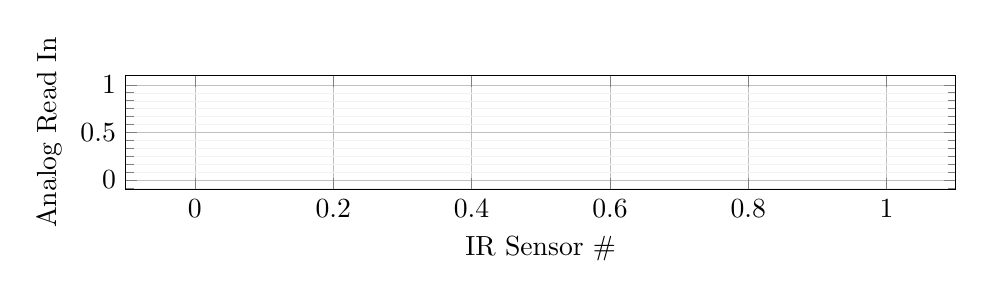
\begin{tikzpicture}
\begin{axis}[
    width=1\textwidth, % Adjust the width as needed
    height=0.25\textwidth, % Adjust the height as needed
    xlabel={IR Sensor \#},
    ylabel={Analog Read In},
    xtick={1, 2, 3, 4, 5, 6, 7}, % Set specific x-axis labels
    legend pos=north west,
    grid=both,
    grid style={line width=.1pt, draw=gray!10},
    major grid style={line width=.2pt,draw=gray!50},
    minor y tick num=5, % This adds the minor grid lines on the y-axis
    minor x tick num=0, % This removes the minor grid lines on the x-axis
    ]
    \IRTrace{green}{Green}{green}
    \IRTrace{blue}{Blue}{blue}
    \IRTrace{red}{Red}{red}
    \IRTrace{yellow}{Yellow}{black}
    \IRTrace{black}{Off}{black}
\end{axis}
\end{tikzpicture}
\caption{IR Calibration Data Based on Tape Color.}
\label{ir-calibration-data}
\end{figure}

\end{document}


\section{Motor Calibration Points}
\label{sc:motor-points}
\documentclass[12pt]{report}
\usepackage{GraphDefinitions}

\begin{document}

\begin{figure}[H]
\centering
\begin{tikzpicture}
    \begin{axis}[
        title = {Speed Percent ($\% \cdot 100$) vs Speed (cm/s)},
        width=1\textwidth, % Make the plot as wide as the subfigure
        height=0.45\textwidth, % Adjust the height for a wide format
        xlabel={Speed (cm/s)},
        ylabel={Speed Percent ($\% \cdot 100$)},
        legend pos=north west,
        ymin = -10,
        grid=both,
        grid style={line width=.1pt, draw=gray!10},
        major grid style={line width=.2pt,draw=gray!50},
        ]
        \MotorTrace{left}{speed_percent}{Left Speed Percent}{red}{solid}        
        \MotorTrace{right}{speed_percent}{Right Speed Percent}{green}{solid}
        \MotorTrace{top}{speed_percent}{Top Speed Percent}{blue}{solid}
        \MotorTrace{bottom}{speed_percent}{Bottom Speed Percent}{black}{solid}
    \end{axis}
\end{tikzpicture}
\label{speed-calibration-data}
\caption{Motor Calibration Data Regarding Speed Percent}
\end{figure}

\vspace{0.5cm} % Space between the subfigures

\begin{figure}[H]
\centering
\begin{tikzpicture}
    \begin{axis}[
        title = {PWM Percent ($\% \cdot 100$) vs Speed (cm/s)},
        width=\textwidth, % Make the plot as wide as the subfigure
        height=0.45\textwidth, % Adjust the height for a wide format
        xlabel={Speed (cm/s)},
        ylabel={PWM Percent ($\% \cdot 100$)},
        ymin = -10,
        legend pos=north west,
        grid=both,
        grid style={line width=.1pt, draw=gray!10},
        major grid style={line width=.2pt,draw=gray!50},
        ]
        \MotorTrace{left}{pwm_percent}{Left PWM Percent}{red}{solid}        
        \MotorTrace{right}{pwm_percent}{Right PWM Percent}{green}{solid}
        \MotorTrace{top}{pwm_percent}{Top PWM Percent}{blue}{solid}
        \MotorTrace{bottom}{pwm_percent}{Bottom PWM Percent}{black}{solid}
    \end{axis}
\end{tikzpicture}
\label{pwm-calibration-data}
\caption{Motor Calibration Data Regarding PWM Percent}
\end{figure}

\end{document}


\end{document}
\documentclass[12pt]{report}
\usepackage{StyleSheets/main}
\begin{document}

\chapter{Diagrams}

\section{Robot Designs}
\label{sc:designs}

\subsection{Design 1}
\begin{figure}[H]
    \centering
    \includegraphics[width=0.5\textwidth]{Images/Designs/Design1.pdf}
    \caption{Design 1 Conceptual Design}
    \label{fig:design1}
\end{figure}

\subsection{Design 2}
\begin{figure}[H]
    \centering
    \includegraphics[width=0.9\textwidth]{Images/Designs/Design2.pdf}
    \caption{Design 2 Conceptual Design}
    \label{fig:design2}
\end{figure}

\subsection{Design 3}
\begin{figure}[H]
    \centering
    \includegraphics[width=0.9\textwidth]{Images/Designs/Design3.pdf}
    \caption{Design 3 Conceptual Design}
    \label{fig:design3}
\end{figure}

\subsection{Design 4}
\begin{figure}[H]
    \centering
    \includegraphics[width=0.9\textwidth]{Images/Designs/Design4.pdf}
    \caption{Design 4 Conceptual Design}
    \label{fig:design4}
\end{figure}

\end{document}
\documentclass[12pt]{report}
\usepackage{StyleSheets/main}
\begin{document}

\pagestyle{code} % Removes footer line 
\thispagestyle{code} % Overrides the chapter "plain" style

\chapter{Code}\label{ap:code}

\section{main.ino}
\lstinputlisting[language=cpp,  caption={main.ino}, label=lst:main-h]{code/main/main.ino}


\section{ObstacleAvoidance.h}
\lstinputlisting[language=cpp,  caption={ObstacleAvoidance.h}, label=lst:obstacleavoidance-h]{code/main/ObstacleAvoidance.h}

\section{PickupPlace.h}
\lstinputlisting[language=cpp,  caption={PickupPlace.h}, label=lst:pickupplace-h]{code/main/PickupPlace.h}

\section{Initialization.h}
\lstinputlisting[language=cpp,  caption={Initialization.h}, label=lst:initialization-h]{code/main/Initialization.h}

\section{LineFollowing.h}
\lstinputlisting[language=cpp,  caption={LineFollowing.h}, label=lst:linefollowing-h]{code/main/LineFollowing.h}

\section{Motion.h}
\lstinputlisting[language=cpp,  caption={Motion.h}, label=lst:motion-h]{code/main/Motion.h}

\section{Sensors}

\subsection{Button.h}
\lstinputlisting[language=cpp,  caption={Button.h}, label=lst:button-h]{code/main/sensors/Button.h}

\subsection{ColorSensor.h}
\lstinputlisting[language=cpp,  caption={ColorSensor.h}, label=lst:colorsensor-h]{code/main/sensors/ColorSensor.h}

\subsection{IRSensorArray.h}
\lstinputlisting[language=cpp,  caption={IRSensorArray.h}, label=lst:irsensorarray-h]{code/main/sensors/IRSensorArray.h}

\subsection{Motor.h}
\lstinputlisting[language=cpp,  caption={Motor.h}, label=lst:motor-h]{code/main/sensors/Motor.h}

\subsection{MWServo.h}
\lstinputlisting[language=cpp,  caption={MWServo.h}, label=lst:mwservo-h]{code/main/sensors/MWServo.h}

\subsection{UltraSonic.h}
\lstinputlisting[language=cpp,  caption={UltraSonic.h}, label=lst:ultrasonic-h]{code/main/sensors/UltraSonic.h}

\section{Controls}
\subsection{PIDController.h}
\lstinputlisting[language=cpp,  caption={PIDController.h}, label=lst:pidcontroller-h]{code/main/controls/PIDController.h}

\subsection{Utils.h}
\lstinputlisting[language=cpp,  caption={Utils.h}, label=lst:utils-h]{code/main/controls/Utils.h}

\section{BoxControl.h}
\lstinputlisting[language=cpp,  caption={BoxControl.h}, label=lst:boxcontrol-h]{code/main/BoxControl.h}


\pagestyle{fancy} % Defaults to normal headers & footers

\end{document}


\end{document}